\section{Learning Outcomes}
\label{Chapter6}

By the end of week 6, you should:

\begin{enumerate}
\item Be familiar with the {\tt csv} module.
\item Be familiar with the \texttt{pandas} module.
\item Be able to perform simple manipulation of pandas databases.
\item Be able to make intermediate level plots (including adding error bars).
\end{enumerate}


\section{Loading CSV files}
\label{sec:csv}

You will be familiar with spreadsheets in Excel. These are more generally (outside the world of Microsoft) described as comma-separated values (or csv) files, in fact you may have seen the ability in Excel to export to a csv file. Python has a built in module for accessing the data in csv files. To import the {\tt csv} module just repeat one of the techniques you used in Section~\ref{modload}.

Remember that you should always load your modules at the start of a set of code (i.e  in the first \texttt{Jupyter} cell) and only load a given module once. Note that, if you are using multiple cells and each one has one or more modules loaded, it'd be worth restarting the kernel and clearing output now and again to clear the memory.

You will now need to download the \texttt{PythonExampleCSVfile1.csv} file in order to complete the exercises below. The file is on Canvas under Week 6.

If you double click on the icon of this file, it opens in Excel or whatever software is your default spreadsheet software. If you do that, you can see the sort of information it contains. This file was generated by a PhD student, and contains real astronomy research data; however, for these exercises, the meaning of the data is irrelevant.

\newpage

\subsection{Specifying Directories}
\label{sec:directories}

When on university computers, the path to a file in Downloads, Desktop, Documents are, respectively:\\
{\tt C://Users/<insert username>/Downloads/<insert filename>}\\
{\tt C://Users/<insert username>/Desktop/<insert filename>}\\
{\tt C://Users/<insert username>/Documents/<insert filename>}\\

For example, if user jb007 wants to load {\tt Python1718exampleCSVfile1.csv} from the Downloads folder, they would do the following

% We should test this
\begin{lstlisting}[style=PY]
In[1]:  # Define the file path as a variable
        path="C://Users/jb007/Downloads/PythonExampleCSVfile1.csv"
        
        # Open the file and do something
        with open(path) as afile:
            #Do something with the file
            pass
\end{lstlisting}

This will be similar on your personal computers but not exactly the same. Have a look at the filepath displayed for the file, and then copy this into the path variable as shown above.
\emph{Within the PIP-Python module, we recommend that you copy any input CSV files
to the same directory as your notebook (this can be done using File Explorer
on a Windows machine, or Finder on a mac).
Doing so means that you do not need to specify the file path in your notebook;
see the next subsection for an example.
This is particularly important when you submit assignments,
as any hard-wired file paths will not work for your marker.}

\subsection{The \texttt{csv} Module}
This example assumes the CSV file is in the same directory where you are running Jupyter.  If you do not know how to copy the .csv into the same directory as your Jupyter notebook, then ask an AT at the next lab session. In the mean time, refer to Section~\ref{sec:directories}.

\begin{lstlisting}[style=PY]
In[1]:  import csv

        with open('PythonExampleCSVfile1.csv','r') as myfile:
        
            # Assign the data in the file to a variable
            mydata = csv.reader(myfile)
            
            # Loop over rows in the dataset
            for myrow in mydata:
                print (myrow)
\end{lstlisting}

Write these statements into a Jupyter cell to make sure they work for you. If you get an error similar to the one below then the .csv file is not in the right directory (ask an AT for help).

\begin{lstlisting}[style=PY_out]
IOError: [Errno 2] No such file or directory: 'PythonExampleCSVfile1.csv'
\end{lstlisting}

Lets go through the above example step by step: 

\begin{itemize}

\item This method of loading data from CSV files uses code blocks (i.e stuff you would indent). 

\item The {\tt with} statement is similar to the {\tt if} statement, and so command lines after that need to be indented.  Think of the {\tt with} statement as meaning {\it 'with this\_item do the following'}. Normally the item being referred to is a file. More detail on \texttt{with} will be presented later in the course.

\item The {\tt open} command then opens the file, which is defined in a string (or you could use a variable that has been set to the filename).

\item The {\tt `r'} statement that comes after the filename will be unfamiliar to you, but is very important. This statement (or equivalent statements) define the {\it mode} of the file. In this case '\texttt{r}' stands for read. Again, more on this later.

\item We then use '\texttt{as myfile}' to assign the  file to the variable \texttt{myfile}.

\item The next line in the code block uses the {\tt csv.reader} function to read in the file to the variable \texttt{mydata}. Then a {\tt for} loop is used to print each row of \texttt{mydata}, by assigning each row, in turn, to the variable {\tt myrow}. The variable names (\texttt{myfile}, \texttt{mydata}, {\tt myrow}) are irrelevant, e.g. even if you changed the code to say '\texttt{mycolumn}', the data would still be read in as rows. 

\item After the {\tt for} loop is finished and the with block has been exited, you cannot try to read in the \texttt{data} variable, as once the file has been read it is closed. Practice making that error now, because it is more than likely you will make that mistake by accident in future, and its good to get familiar with the error codes, so you can diagnose them quickly.

\end{itemize}

To be able to use all the data within the CSV file, we have to assign the data to lists. The contents of the file \texttt{PythonExampleCSVfile1.csv} can be seen in Table.\ref{tab:s4csv}.

\begin{table}[H]
\begin{center}
\caption{Contents of PythonExampleCSVfile1.csv}
\begin{tabular}{|l|l|}
\hline
Column A:& name\\\hline
Column B:& redshift\\\hline
Column C:& mean-$x$\\\hline
Column D:& mean-$x$ minus delta-$x$\\\hline
Column E:& mean-$x$ plus delta-$x$\\\hline
Column F:& mean-$y$\\\hline
Column G:& mean-$y$ minus delta-$y$\\\hline
Column H:& mean-$y$ plus delta-$y$\\\hline
\end{tabular}
\label{tab:s4csv}
\end{center}
\end{table}\vspace*{-3ex}

The use of the \texttt{csv} module then requires you to iterate through each row and column and assign the data to lists... This is computationally expensive to do yourself when the files get large (~GB), and tedious at best... Fortunately there is a better way to load data into Python! 

\begin{tcolorbox}[colback=red!5!white,colframe=red!75!black]
\subsubsection{Variable Names}

Please be careful when naming variables for files - if you try to use a variable like \texttt{list} or \texttt{file}, you will be overwriting a built-in python function. As a general rule, if your variable turns green in \texttt{Jupyter} - do not use it!

If you accidentally do this - restart your kernel.
\end{tcolorbox}

\newpage

\subsection{The \texttt{pandas} Module}

Pronounced just like the adorable black and white bears, this module is one of the easiest ways to start playing around with data in Python. Lets start by loading the csv into a pandas data frame (think of a data frame exactly like a Sheet in Excel or Google Docs). 

\begin{lstlisting}[style=PY]
In[2]:  import pandas as pd
        
        # Open the csv file as a dataframe
        df = pd.read_csv("PythonExampleCSVfile1.csv", index_col=None)
\end{lstlisting}

The standard abbreviation for the \texttt{pandas} is \textit{pd}, similar to how the \texttt{numpy} module from last week was \texttt{np}.

To read in the csv file, we use the aptly named method \texttt{read\_csv}. This method can take only one argument, the csv filename, however, we should also tell \texttt{pandas} not to read the first column as an index column. Think of the index column as the row numbers in Excel, pandas allows both \texttt{int} and \texttt{str} indices, but for now we will tell pandas that our file doesn't have an index column already; \texttt{pandas} will create one for us using integers from 0 to the number of rows in the csv. (Note: \texttt{pandas} assumes this by default, however it is incredibly useful for readability if this argument is explicitly given. This is true of any argument to any function, even if using the default value it can be very helpful for understanding to explictly state the arguments.)

Another bonus of using \texttt{pandas} is that it assumes the first row in the csv are the column names - and automatically uses them. Take a look with the \texttt{columns} attribute.

\begin{lstlisting}[style=PY]
In[3]:  df.columns
\end{lstlisting}
\begin{lstlisting}[style=PY_out]
Out[3]: Index(['Name', 'Redshift', 'Mean_X', 'Mean_x_minus_delta',
        'Mean_x_plus_delta','Mean_y', 'Mean_y_minus_delta',
        'Mean_y_plus_delta'], dtype='object')
\end{lstlisting}

\noindent We can also take a look at the data frame using the \texttt{head} function to get the first N rows (here 10).

\begin{lstlisting}[style=PY]
In[4]:  df.head(10)
\end{lstlisting}

And because of the way \texttt{jupyter} and pandas work well together, you should get a nice table shown that should look something like Figure \ref{fig:df_head}.

\begin{figure}[H]
	\centering
	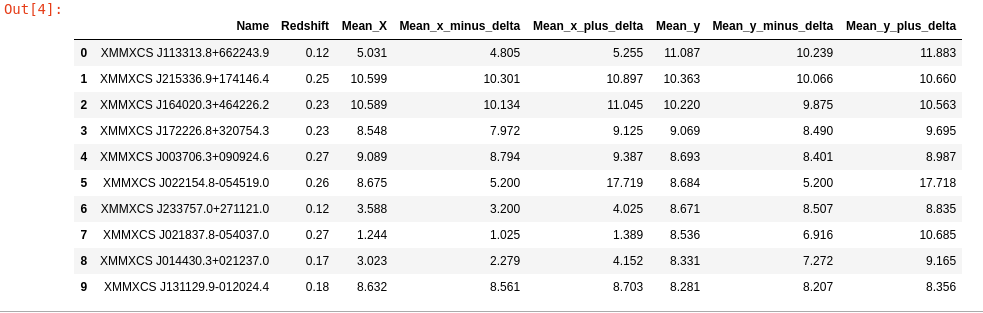
\includegraphics[scale=0.45]{Pictures/df_head.png}
\caption{Output of df.head(10) showing the first 10 rows in PythonExampleCSVfile1.csv}
\label{fig:df_head}
\end{figure}

\newpage

If we want to plot just the \textit{Mean\_X} and \textit{Mean\_y} columns against each other, we can use the column names similarly to how we have previous used functions within modules.

\begin{lstlisting}[style=PY]
In[5]:  import matplotlib.pyplot as plt

        # Set up plot
        plt.figure()
        
        # Plot a scatter of the mean x and y data
        plt.scatter(df.Mean_X, df.Mean_y, marker=".")
        
        # Label axes
        plt.xlabel("Mean X")
        plt.ylabel("Mean Y")
        
        plt.show()
\end{lstlisting}

\begin{figure}[H]
	\centering
	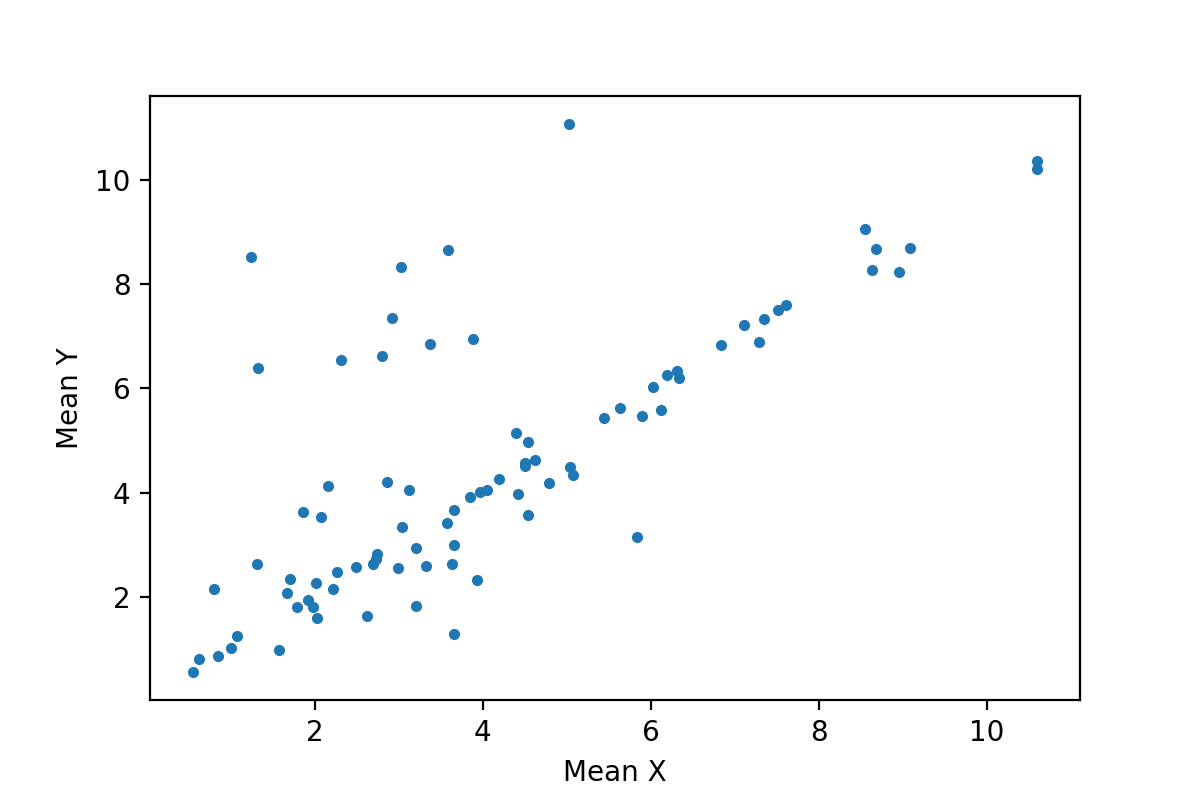
\includegraphics[scale=1]{Pictures/Week6_x_v_y.png}
\caption{Scatter plot of the Mean X and Y values.}
\label{fig:df_head}
\end{figure}

\newpage

If we want to just get the values from a column into a data structure we have worked with before, we can do the following:

\begin{lstlisting}[style=PY]
In[6]: df.Mean_X.values.tolist()
\end{lstlisting}
\begin{lstlisting}[style=PY_out]
Out[6]: [5.031000000000001,
         10.599,
         10.589,
         8.548,
         9.089,
         8.675,
         3.588,
         1.244,
         3.023,
         8.632,
         ...
\end{lstlisting}


Where \texttt{values} gets all the values in the column Mean\_X, and \texttt{tolist()} converts the column into a list. 

If we want to grab a specific row within the data frame, we can use the function \texttt{loc}, which uses the index (in our case just row numbers starting at 0).

\begin{lstlisting}[style=PY]
In[7]:  print(df.loc[0])
        print()  # create a blank line in output
        print(df.loc[50])
        print()  # create a blank line in output
        print(df.loc[50,"Mean_X"])
\end{lstlisting}

\begin{lstlisting}[style=PY_out]
        Name                  XMMXCS J113313.8+662243.9
        Redshift                                   0.12
        Mean_X                                    5.031
        Mean_x_minus_delta                        4.805
        Mean_x_plus_delta                         5.255
        Mean_y                                   11.087
        Mean_y_minus_delta                       10.239
        Mean_y_plus_delta                        11.883
        Name: 0, dtype: object
        
        Name                  XMMXCS J004252.6+004303.1
        Redshift                                   0.27
        Mean_X                                    2.072
        Mean_x_minus_delta                        1.496
        Mean_x_plus_delta                         3.187
        Mean_y                                    3.527
        Mean_y_minus_delta                        3.002
        Mean_y_plus_delta                         4.525
        Name: 50, dtype: object
        
        2.072
\end{lstlisting}

\vspace{0.1cm}

Here we see all the information for the first row (row 0) in the first print statement; use a lazy way of forcing a new line by calling the print function without any arguments; see all the information for the 51st row and then only print the value from the ``Mean\_X'' column of the 51st row by passing the column name to the \texttt{loc} function as the second argument.

The \texttt{loc} function also allows slicing, similar to the way you have previously done for lists.

\begin{lstlisting}[style=PY]
In[8]:  print(df.loc[0:2,"Mean_X"])
        print(df.loc[0:2,"Mean_X"].values.tolist())
\end{lstlisting}
\begin{lstlisting}[style=PY_out]
        0     5.031
        1    10.599
        2    10.589
        Name: Mean_X, dtype: float64
        
        [5.031000000000001, 10.599, 10.589]
\end{lstlisting}

Where we have used the \texttt{values.tolist()} functions to turn 3 rows from the column into a list, which we are more familiar with.

It is encouraged that you use the \textbf{help} function to look through \texttt{pd.DataFrame}, which will tell you about all the other functions which can be used. In particular the \texttt{shape} function can be used to tell you how many rows, and how many columns are in the data frame.

\begin{lstlisting}[style=PY]
In[9]:   df.shape
\end{lstlisting}
\begin{lstlisting}[style=PY_out]
Out[9]: (84,8)
\end{lstlisting}

The output, \textbf{(84,8)}, tells us that our \texttt{DataFrame} (\texttt{df}) has 84 rows and 8 columns. Note that this means we actually have 84 rows, not 83 rows and the columns names; i.e. the column names \textbf{do not} count as a row.

You can apply all operators to the columns, and pandas will perform the operation on each row at a time. You can then store the results back into the data frame in the same way as a dictionary.

\begin{lstlisting}[style=PY]
In[10]: # Define new columns containing the data produced by an operation
        df["Mean_X_upper"] = df.Mean_x_plus_delta - df.Mean_X
        df["Mean_X_lower"] = df.Mean_X - df.Mean_x_minus_delta
        
        # Output the first row after making these changes
        df.loc[0]
\end{lstlisting}
\begin{lstlisting}[style=PY_out]
Out[10]:    Name                  XMMXCS J113313.8+662243.9
            Redshift                                   0.12
            Mean_X                                    5.031
            Mean_x_minus_delta                        4.805
            Mean_x_plus_delta                         5.255
            Mean_y                                   11.087
            Mean_y_minus_delta                       10.239
            Mean_y_plus_delta                        11.883
            Mean_X_upper                              0.224
            Mean_X_lower                              0.226
            Name: 0, dtype: object
\end{lstlisting}


\subsubsection{Saving your DataFrame}
Before we move onto the exercises and analysing the data from the csv, you may want to save your dataframe in some manner. To do so you can write the DataFrame back to a csv - creating a hard copy so to speak. This way - if you screw up - you can load back in the data from a previous state. For this course, you will rarely be working on sufficiently large data to warrant such an approach, but it is useful.

To save as a csv file simply call the \texttt{to\_csv} method.

\begin{lstlisting}[style=PY]
In[11]  df.to_csv("Week6_with_errors.csv")
\end{lstlisting}

\subsection{Exercises}
\label{ex1}
Have you managed to get the first 10 entries of the astronomy file to print out? If not, don't move on until you've done it.

\begin{enumerate}
    \item Week6Basic - Write a code to view and create columns in a DataFrame.
    \begin{enumerate}
        \item[a)] Print the 50th, 72nd and 9th rows, including all their columns.
        \item[b)] In one code line, print the Mean\_y values for \textbf{rows} 62-71.
        \item[c)] Add two new columns to your data frame similar to the Mean\_X\_upper and Mean\_X\_lower example above for y. (You should also have done this for X, if not, do this now).
        \item[d)] Save the updated DataFrame with the new columns to a csv file.
        \item[e)] Read the csv you just created back into a new DataFrame, and have a look - what do you now notice? (If you're not sure look at pd.read\_csv with the help function, and if you're still not sure ask an AT)
    \end{enumerate}
\end{enumerate}

\newpage

\section{Plotting data points and error bars}
\label{plotdataerror}

\subsection{Data points}
\label{datapoints}

Last week you were introduced to some basic plotting with the matplotlib library. Already this week we have used an example of the scatter plot, and for the rest of this week we will be going through some basic tools for handling and fitting data in python.

To begin with we are going to create some random data, and create a scatter plot. Unlike last week's section on this, here we will use the \texttt{numpy.random} module. This is covered again in Sec. \ref{sec:numpyrandom}.

\begin{lstlisting}[style=PY]
In[12]  from numpy.random import default_rng

        # Set the seed so that we all get the same result.
        rng = default_rng(12345)
        
        # Create random data for x and y
        x_data = rng.random(100)
        y_data = rng.random(100)
        
        # Plot the random data
        plt.figure()
        plt.scatter(x_data,y_data,marker='x',color='r')
        plt.show()
\end{lstlisting}

Hopefully you should get something that looks like Figure~\ref{fig:random_scatter}.

\begin{figure}[H]
	\centering
	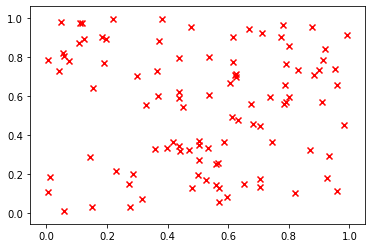
\includegraphics[scale=0.75]{Pictures/Week6_random_scatter.png}
\caption{Scatter Plot result of random points.}
\label{fig:random_scatter}
\end{figure}

You are welcome to (and for some of the exercises required to) use the table below for reference. It contains a selection of possible marker and color options available to most \texttt{matplotlib} functions.

\begin{table}[H]
\begin{center}
\begin{tabular}{|l | p{2cm}|}
\hline
b & blue\\\hline
g & green\\\hline
r & red\\\hline
c & cyan\\\hline
m & magenta\\\hline
y & yellow\\\hline
k & black\\\hline
w & white \\\hline
\end{tabular}
\hspace{4ex} 
\begin{tabular}{|l | p{3cm}|}
\hline
s & square\\\hline
p & pentagon\\\hline
\texttt{*} & star\\\hline
h & hexagon\\\hline
o & circle\\\hline
+ & plus\\\hline
x & cross\\\hline
D & diamond\\\hline
- & line\\\hline
\end{tabular}
\end{center}
\caption{A reference for plotting data points with markers and colours.}
\label{tab:plte}
\end{table}

\subsection{Plotting error bars}
\label{errorbar}

{\tt Matplotlib} allows you to plot error bars using the {\tt errorbar} function in place of {\tt plot} or \texttt{scatter}. Here we will show you a few examples using {\tt errorbar}.

\begin{itemize}

\item {\bf Example 1:} the error bars are symmetrical and the same on each point, see Figure~\ref{fig:peb1}.

\begin{lstlisting}[style=PY]
In[13]  plt.figure()
        plt.errorbar(x_data, 
                     y_data, 
                     yerr=0.05, 
                     xerr=0.05, 
                     fmt='ro', 
                     ecolor="k", 
                     capsize=2)
        plt.show()
\end{lstlisting}

\begin{figure}[H]
	\centering
	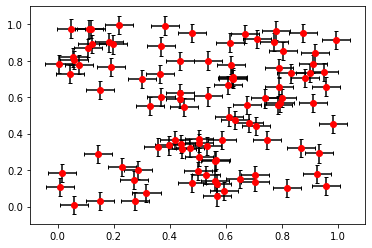
\includegraphics[scale=0.75]{Pictures/Week6_random_scatter_werrors.png}
\caption{Scatter Plot result of random points with error bars.}
\label{fig:peb1}
\end{figure}

For this example, we have used the \texttt{yerr} and \texttt{xerr} arguments to plot symmetric error-bars on each point. \texttt{fmt} is the marker format argument, where \texttt{r} denotes the color red, and the \texttt{o} tells \texttt{errorbar} to use circles as markers (these can be exchanged for the \texttt{color} and \texttt{marker} respectively). For the errorbar color, we use the argument \texttt{ecolor}, which uses the same color names as the normal plotting functions you've already come across. \texttt{capsize} is an optional choice, that sets the size of the little orthogonal bars on the end of each error bar.

\item {\bf Example 2:}  the error bars are symmetrical, but in the $x$-direction they are different for each point, see Figure~\ref{fig:peb2}.

\begin{lstlisting}[style=PY]
In[14]  # Get random errors for the x axis 
        xerr = rng.random(100)/10
        
        # Plot the result
        plt.figure()
        plt.errorbar(
                    x_data,
                    y_data,
                    yerr=0.05,
                    xerr=xerr,
                    fmt='ro',
                    ecolor="k",
                    capsize=2)
        plt.show()
\end{lstlisting}

\begin{figure}[H]
	\centering
	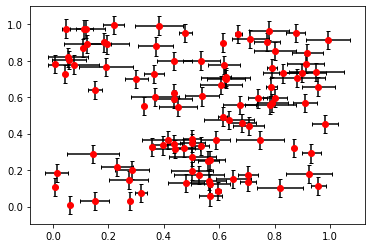
\includegraphics[scale=0.75]{Pictures/Week6_random_scatter_w_rerrors.png}
\caption{Scatter Plot result of random points with constant y and random symmetric x error bars.}
\label{fig:peb2}
\end{figure}

\newpage

\item {\bf Example 3:} the error bars are not symmetrical (they have different upper and lower values) and differ for each point. See Figure~\ref{fig:peb3}.

\begin{lstlisting}[style=PY]
In[15]  # Get random upper and lower errors for both x and y
        xerr = [rng.random(100)/10,
                rng.random(100)/10]
        yerr = [rng.random(100)/10,
                rng.random(100)/10]
                
        # Plot the result
        plt.figure()
        plt.errorbar(
                    x_data,
                    y_data,
                    yerr=yerr,
                    xerr=xerr,
                    fmt='ro',
                    ecolor="k",
                    capsize=2)
        plt.show()
\end{lstlisting}

\begin{figure}[H]
	\centering
	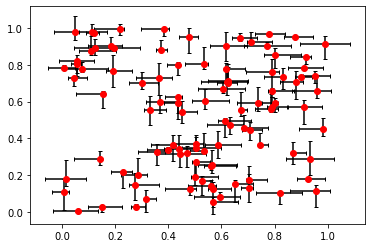
\includegraphics[scale=0.75]{Pictures/Week6_random_scatter_w_rerrors2.png}
\caption{Scatter Plot result of random points with random error bars.}
\label{fig:peb3}
\end{figure}

\end{itemize}

\subsubsection{Exercises (with worked answers)}

See Section~\ref{FigureSection} for worked answers.

\begin{enumerate}
\item Create a range from $0$ to $5$ with steps of $0.01$ and assign to variable t. Then apply the function $f(t)= t\sin(10t)$ and plot with data points as yellow stars.
\item Plot the following data with its associated errors, with the data point as blue diamonds and error bar colour as green:\\
y=1.474, 1.021, 0.506\\
x=0.00400, 0.00270, 0.00120\\
x\_lower=0.001, 0.0002, 0.0003\\
x\_upper=0.001, 0.001, 0.001\\
y\_lower=0.003, 0.002, 0.003\\
y\_upper=0.004, 0.004, 0.01
\item Using your DataFrame from Section~\ref{ex1}, plot X against Y with your calculated error bars. Limit the X axis between 0 and 12
\end{enumerate}


\subsubsection{Exercises (other)}

\begin{enumerate}
    \item Plot $y=\sin(x)$ with the x being a range from $0$ to $5$ with increments of $0.1$, with y-error = $0.5$, x-error = $0$.
    \item Plot $y=\sin(x)$ with the x being a range from $0$ to $5$ with increments of $0.1$, with y-upper-error = $+0.5$, y-lower-error = $-2$, x-error = $0$.  With the data points being in red and the error bar colour green.
    \item Using a file containing Exoplanet data \texttt{PythonExampleCSVfile2.csv}, plot Semi-Major axis (AU) vs. Orbital Period (day). Apply associated errors, have the error bars as black and data points as red pluses. Label axis and add a title 'Exoplanet data'. Table \ref{tab:exop} shows the layout of the csv file.
\end{enumerate}


\begin{table}[H]
\begin{center}
\caption{Contents of exoplanets data csv}
\begin{tabular}{|l|l|}
\hline
Column A:& name\\\hline
Column B:& X (Semi-Major axis)\\\hline
Column C:& X error\\\hline
Column D:& Y (Orbital period)\\\hline
Column E:& Y lower error bound\\\hline
Column F:& Y upper error bound\\\hline
\end{tabular}
\label{tab:exop}
\end{center}
\end{table}\vspace*{-3ex}

\newpage

\section{Fitting straight lines to data points}
\label{linefit}

There are numerous ways of fitting lines to data in \texttt{Python}. A more sophisticated method will be covered in Chapter \ref{chap:sci} but we will show here a simple method that utilises the \texttt{numpy.polynomial} module. This module allows one to fit polynomials of varying order.  The example below shows how to fit a 1D polynomial.

\begin{lstlisting}[style=PY]
  In[16]  from numpy.polynomial import Polynomial
        # Mock data to fit
        x = [1, 2, 3, 4, 5, 6, 7, 8] 
        y = [1.5,2,3.6,4,5,6.7,7.45,8.1]
        
        # Using numpy.polynomial, fit the line with a first order polynomial
        p = Polynomial.fit(x, y, deg=1)
        
        # Some x values to plot the fit with
        x_fit = np.linspace(0, 10, 100)
        
        # And plot the results
        plt.figure()
        plt.plot(x, y, 'ro', label='Data' )
        plt.plot(x_fit, p(x_fit), label='Best fit line') 
        plt.legend(loc='best') 
        plt.show()
\end{lstlisting}

\begin{figure}[H]
	\centering
	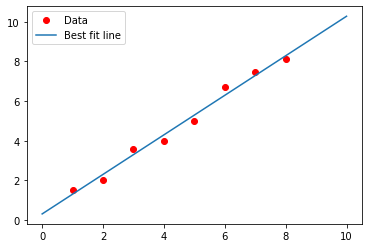
\includegraphics[scale=0.75]{Pictures/linefit.png}
\caption{Plot result from fitting the mock data in Section~\ref{linefit}}
\label{fig:bf1}
\end{figure}

See Fig.\ref{fig:bf1} for the output. Note that here we are using the {\tt label} argument to add labels to the fit and data points, and the \texttt{legend} method to add a legend to the plot with these labels. Lets go through the rest of the example:

\begin{itemize}


\item We define some \texttt{x} and \texttt{y} data as lists. 

\item Next we call the \texttt{Polynomial.fit} function which uses the raw \texttt{x} and \texttt{y} data to compute an instance {\tt p} of a Polynomial of degree 1.
If you wish to see the output of \texttt{poly1d} use \texttt{print(p)}, and the following output should be shown \texttt{4.79 + 3.49 x}.

\item The \texttt{linspace} function creates an array to evaluate the fit at (variable \texttt{p} contains the fitting function). The general syntax for \texttt{linspace} is \texttt{linspace(a,b,n)}, where the array runs from \texttt{a} to \texttt{b} (\textbf{inclusive of \texttt{b}}) using an \texttt{n} number of points. 

\item The \texttt{legend} command in the next line uses the labels from the plots and creates a legend. We use the \texttt{loc} argument to define the legend's location, in this case \texttt{'best'} means it places the legend in the best location. The default location is indeed \texttt{'best'}, but as previously mentioned it's good to be specific!

\item The final command shows the plot.

\end{itemize}

\subsection{Exercises}

\begin{enumerate}
    \item Plot x vs. y with red circles as data points. Use \texttt{polyfit} to fit a line of best fit as a green dashed line and add a legend. Hint: For dashed line use \texttt{\color{mygreen}'--'}. .\\ 
    x = 0.0, 0.5, 1.0, 1.5, 2.0, 2.5, 3.0, 3.5, 4.0, 4.5, 5.0, 5.5, 6.0, 6.5, 7.0, 7.5, 8.0, 8.5, 9.0, 9.5.\\ 
    y = -0.23, 0.53, 3.8, -3.16, -7.45, -11.76, 2.38, -14.65, 12.64, -13.2, 2.99, 21.08, -3.48, 26.74, -19.49, 8.03, -4.63, -49.06, 29.73, 54.69
    \item Fitting noisy data:
        \begin{enumerate}
            \item[a)] Plot $f(x)=2x^2+6$ in the range $x\in [-5,5]$. 
            \item[b)] Add random Gaussian noise to $f(x)$ with $\mu=0,\sigma=|x|$ without using loops.
            \item[c)] Fit a 2nd order polynomial to your altered $f(x)$.
            \item[4)] Plot the residuals between your fit and $f(x)$.
        \end{enumerate}
\end{enumerate}


% --------------------------------------- %

\newpage

\section{Answers to Exercises from Sec~\ref{errorbar}}
\label{FigureSection}

This section assumes a blank notebook for each answer. You will not need to import the modules every time.

\begin{lstlisting}[style=PY]
In[1]   import matplotlib.pyplot as plt
        import numpy as np
        
        # store values as asked
        t = np.arange(0,5,0.01)
        
        # Create the desired expanding sine wave
        f = lambda t: t*np.sin(10*t)
        
        # Finally plot the function as yellow stars
        plt.figure()
        plt.scatter(t, f(t),marker='*',color='yellow')
        plt.show()
\end{lstlisting}

\begin{lstlisting}[style=PY]
In[1]   import matplotlib.pyplot as plt
    
        # Store the data from the question as lists
        y=[1.474, 1.021, 0.506]
        x=[0.00400, 0.00270, 0.00120]
        xlower=[0.001, 0.0002, 0.0003]
        xupper=[0.001, 0.001, 0.001]
        ylower=[0.003, 0.002, 0.003]
        yupper=[0.004, 0.004, 0.01]
        
        # Plot with errors as blue diamonds, and green error bars.
        plt.figure()
        plt.errorbar(
                x,
                y,
                xerr=[xlower,xupper],
                yerr=[ylower,yupper],
                fmt='bD',
                ecolor='g',
                capsize=2)
        plt.show()
\end{lstlisting}

\newpage

\begin{lstlisting}[style=PY]
In[1]   import pandas as pd
        import matplotlib.pyplot as plt
        
        # Load in the data
        df = pd.read_csv("PythonExampleCSVfile1.csv",index_col=None)
        
        # Calculate the upper and lower errors
        df["Mean_X_upper"] = df.Mean_x_plus_delta - df.Mean_X
        df["Mean_X_lower"] = df.Mean_X - df.Mean_x_minus_delta
        df["Mean_y_upper"] = df.Mean_y_plus_delta - df.Mean_y
        df["Mean_y_lower"] = df.Mean_y - df.Mean_y_minus_delta
        
        # Finally plot the results
        # Note here that .T simply transposes the result, but any
        # other method is just fine (even calling each column
        # individually is valid)
        plt.figure()
        plt.errorbar(
                df.Mean_X,
                df.Mean_y,
                xerr=df[["Mean_X_lower","Mean_X_upper"]].values.T,
                yerr=df[["Mean_y_lower","Mean_y_upper"]].values.T,
                fmt='bo',
                ecolor="k",
                capsize=3)
        plt.xlim(0,12)
        plt.show()
\end{lstlisting}


